\documentclass{beamer}
\usetheme{Madrid}

\usepackage{graphicx}
\usepackage{tabularx}
\usepackage{subfig}
%\usepackage{biblatex}
%\usepackage{cite}
\usepackage{natbib}

\title[CDT]{Constrained Delaunay Tetrahedralization(CDT) for applications in Nuclear reactor component modelling}
\author{Pranav Kant Gaur}
\institute[BARC, India]{Computer Division, \newline Bhabha Atomic Research Centre, Mumbai, India}
\titlegraphic{
\includegraphics[width=2cm, height=2cm]{figures/barc_logo.jpg}}
\date{}

\begin{document}
%%%%%%%%%%%%%%%%%%%%%%%%%%%%%%%%%%%%%%%%%%%%%%%%%%%%%%%%%%%%%%%%%%%%%%%%%%%%%%%%%%%%%%%%%%%%%%%%%%%%%%%
	\begin{frame}
		\titlepage
	\end{frame}	
%%%%%%%%%%%%%%%%%%%%%%%%%%%%%%%%%%%%%%%%%%%%%%%%%%%%%%%%%%%%%%%%%%%%%%%%%%%%%%%%%%%%%%%%%%%%%%%%%%%%%%%
	\begin{frame}
		\frametitle{Motivation}
			\begin{itemize}
				\item CFD analysis for Nuclear reactor component modelling:
					\begin{itemize}
						\item Designing reactor core:
							\begin{figure}
								\begin{tabularx}{\linewidth}{@{}cXX@{}}
									\begin{tabular}{c c c}
										\hspace{-2cm}\subfloat[]{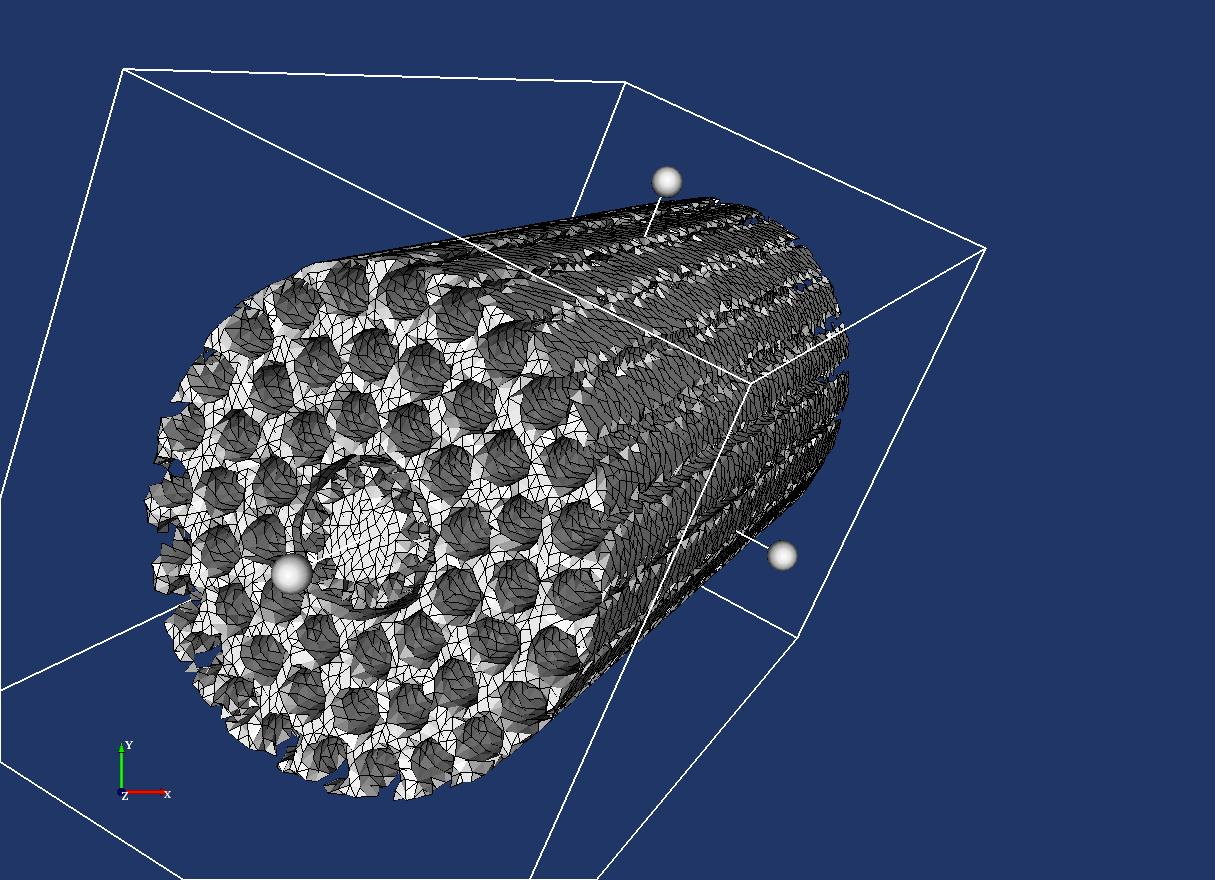
\includegraphics[width=4cm, height=3cm]{figures/fuelView1.jpg}} &
										\subfloat[]{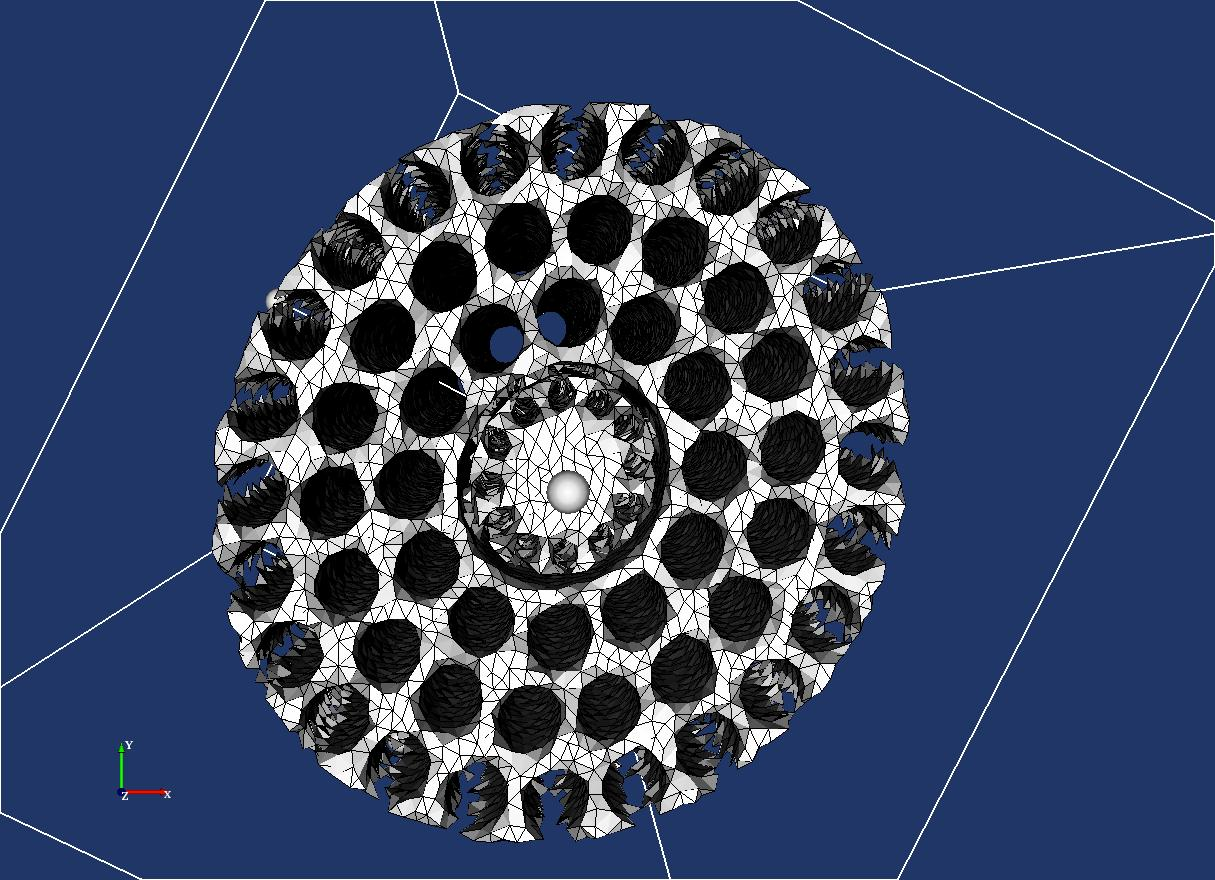
\includegraphics[width=4cm, height=3cm]{figures/fuelView2.jpg}} &
										\subfloat[]{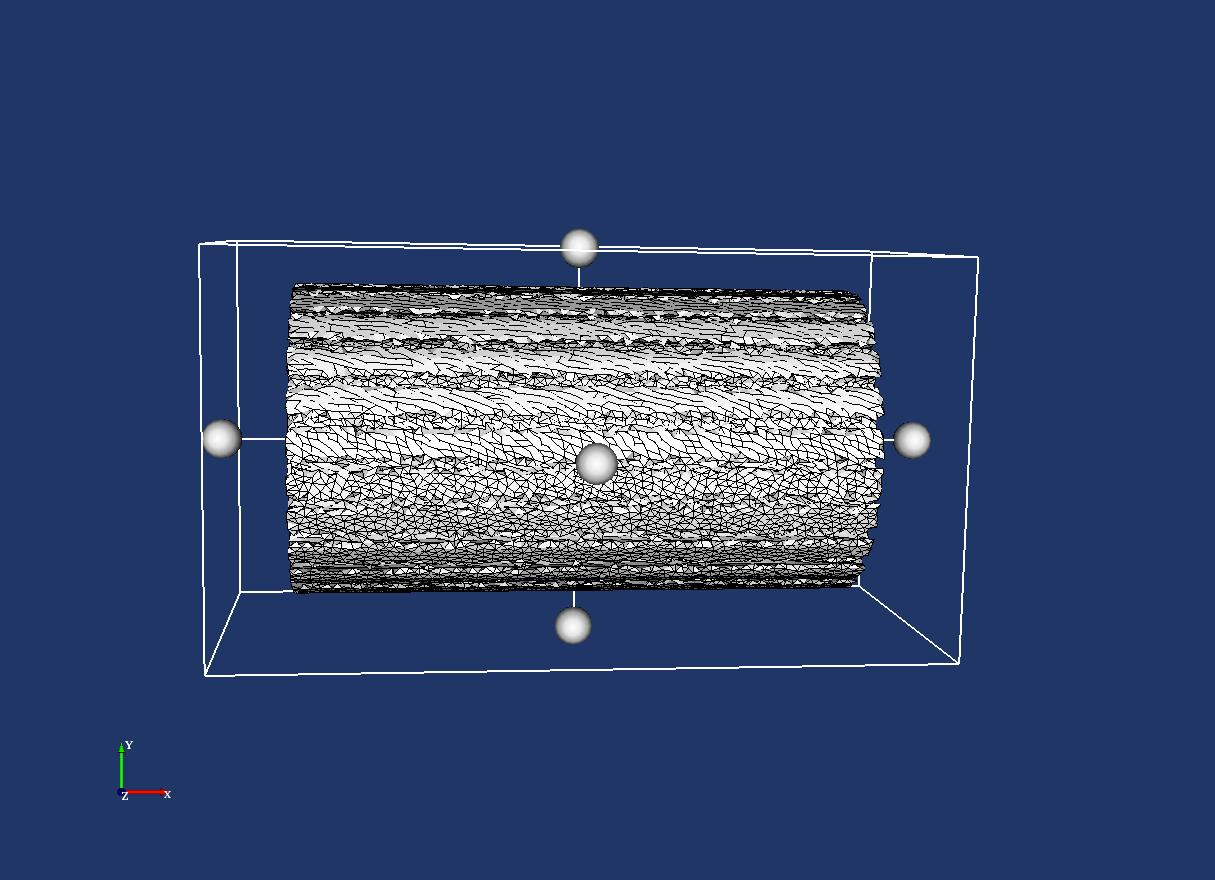
\includegraphics[width=4cm, height=3cm]{figures/fuelView3.jpg}} \\
									\end{tabular}
								\end{tabularx}	
								\caption{Fuel bundle}
							\end{figure}	
					\end{itemize}		
			\end{itemize}
	\end{frame}
%%%%%%%%%%%%%%%%%%%%%%%%%%%%%%%%%%%%%%%%%%%%%%%%%%%%%%%%%%%%%%%%%%%%%%%%%%%%%%%%%%%%%%%%%%%%%%%%%%%%%%%
	\begin{frame}
		\frametitle{Motivation(contd.)}
			\begin{itemize}
				\item Anupravaha
					\begin{itemize}
						\item General purpose CFD solver over hybrid unstructured grid.
						\item Collaboration project between BARC and other academic institutions.
						\item Integrated mesh generation and CFD solver:
							\begin{itemize}
								\item Currently, no open source software  with iterative feedback based hybrid mesh generation capability.
								\item Need to have tighter control over configurability of mesh generation and solver tools.	
							\end{itemize}	
					\end{itemize}		
			\end{itemize}		
	\end{frame}	
%%%%%%%%%%%%%%%%%%%%%%%%%%%%%%%%%%%%%%%%%%%%%%%%%%%%%%%%%%%%%%%%%%%%%%%%%%%%%%%%%%%%%%%%%%%%%%%%%%%%%%%
	\begin{frame}	
		\frametitle{Motivation(contd.)}	
			\begin{itemize}
				\item Resulting mesh should have elements suitable for finite element calculations:
					\begin{itemize}
						\item Constrained Delaunay Tetrahedralization is optimal domain discretization approach for Finite element applications \cite{schewFiniteElements}.
							\begin{itemize}
								\item Preserves input domain in output mesh.
								\item Shares characterstics with Delaunay triangulation \cite{schewCDTExistence}	
								\item Maximizes minimum dihedral angle(\textit{Delaunay property}) \cite{schewFiniteElements}.
							\end{itemize}
					\end{itemize}		
			\end{itemize}		
	\end{frame}
%%%%%%%%%%%%%%%%%%%%%%%%%%%%%%%%%%%%%%%%%%%%%%%%%%%%%%%%%%%%%%%%%%%%%%%%%%%%%%%%%%%%%%%%%%%%%%%%%%%%%%%%
	\begin{frame}
		\frametitle{Constrained Delaunay Tetrahedralization}
			\begin{itemize}
				\item A simplical complex is \textit{constrained Delaunay} if there exist a circumsphere which encloses no other \textit{visible} point inside it.[FIGURE???]
				\item Constrained Delaunay Tetrahedralization is a simplical complex of constrained Delunay cells.
			\end{itemize}
			\begin{}
	\end{frame}	
%%%%%%%%%%%%%%%%%%%%%%%%%%%%%%%%%%%%%%%%%%%%%%%%%%%%%%%%%%%%%%%%%%%%%%%%%%%%%%%%%%%%%%%%%%%%%%%%%%%%%%%%%
	\begin{frame}
		\frametitle{Theoretical underpinnings}
			\begin{itemize}
				\item	Schewchuck's CDT existence theorem \cite{schewCDTExistence}:
					\begin{itemize}
						\item If X is edge protected then CDT of X exists.[ELABORATE??]	
					\end{itemize}		
				\item	Hang Si's Theorem \cite{hangSiMeshingPLCByCDT}
					\begin{itemize}
						\item If X has no local degeneracy and DT of X contains all segments of X, then CDT of X exists.[ELABORATE???] 
					\end{itemize}		
			\end{itemize}		
	\end{frame}	
%%%%%%%%%%%%%%%%%%%%%%%%%%%%%%%%%%%%%%%%%%%%%%%%%%%%%%%%%%%%%%%%%%%%%%%%%%%%%%%%%%%%%%%%%%%%%%%%%%%%%%%%%
	\begin{frame}
		\frametitle{Algorithm} 
			\begin{itemize}
				\item Transform X into an edge protected \textit{topologically equivalent} X':	
				\begin{itemize}
					\item Compute initial Delaunay Tetrahedralization	
					\item Recover constraint segments
					\item Remove local degeneracies
				\end{itemize}
				\item Recover constraint facets
			\end{itemize}		
	\end{frame}
%%%%%%%%%%%%%%%%%%%%%%%%%%%%%%%%%%%%%%%%%%%%%%%%%%%%%%%%%%%%%%%%%%%%%%%%%%%%%%%%%%%%%%%%%%%%%%%%%%%%%%%%%
	\begin{frame}
		\frametitle{Implementation}
			\begin{itemize}
				\item CDTGenerator class{UML diagram class????}:
					\begin{itemize}
						\item Data members{Populate???}
						\item Member functions:{Populate???}	
					\end{itemize}		
				\item Unit tests using Google test
				\item Doxygen inline code documentation
				\item Continous integration testing on Travis CI	
				\item Github repository[REFERENCE LINK???]	
			\end{itemize}
	\end{frame}	
%%%%%%%%%%%%%%%%%%%%%%%%%%%%%%%%%%%%%%%%%%%%%%%%%%%%%%%%%%%%%%%%%%%%%%%%%%%%%%%%%%%%%%%%%%%%%%%%%%%%%%%%%
	\begin{frame}
		\frametitle{Results} 	
	\end{frame}	
%%%%%%%%%%%%%%%%%%%%%%%%%%%%%%%%%%%%%%%%%%%%%%%%%%%%%%%%%%%%%%%%%%%%%%%%%%%%%%%%%%%%%%%%%%%%%%%%%%%%%%%%%
	\begin{frame}
		Thank you all!!{LARGE FONT??????}
	\end{frame}	
%%%%%%%%%%%%%%%%%%%%%%%%%%%%%%%%%%%%%%%%%%%%%%%%%%%%%%%%%%%%%%%%%%%%%%%%%%%%%%%%%%%%%%%%%%%%%%%%%%%%%%%%%
\bibliography{INRIAbib}
\bibliographystyle{plain}
\end{document}
